\documentclass{llncs}
\usepackage[T1]{fontenc}
\usepackage[utf8]{inputenc}
\usepackage{lmodern}
\usepackage{graphicx,booktabs,tabularx,amsmath,amssymb,tikz,url}
\usetikzlibrary{arrows.meta}
\usepackage[hidelinks]{hyperref}
\newcolumntype{Y}{>{\raggedright\arraybackslash}X}
\begin{document}
\pagestyle{empty}
\title{XBone-Net: Class-Aware Vision--Language Adaptation for Musculoskeletal Radiograph Classification}
\author{Nguyen Van Le Ba Thanh \and Nguyen Gia Kiet \and Ly Quoc Ngoc \and Do Thi Thanh Ha}
\institute{Faculty of Information Technology, University of Science,\\
Vietnam National University Ho Chi Minh City, Ho Chi Minh City, Vietnam}
\maketitle
\thispagestyle{empty}

\begin{abstract}
Musculoskeletal radiograph classification combines a long-tailed label distribution with clinical context that is difficult to recover from image appearance alone. Medical vision--language pretraining has improved representation transfer, but its benefits do not directly establish how to adapt a large model to a small radiograph--history dataset or whether additional fusion components are justified. We present XBone-Net, a two-phase adaptation framework built on BiomedCLIP. The offline stage first learns class-aware soft image--text matching through low-rank adapters, then optimizes bidirectional global-to-local cross-attention and a linear classifier. Online prediction uses a radiograph and clinical history with fixed model parameters. Experiments use three training seeds on CTCH, comprising 3,249 pairs from 22 classes, and BTXRD, comprising 3,746 radiographs from 10 classes with metadata-derived text. XBone-Net achieves Macro-F1 scores of $0.5727\pm0.0193$ and $0.6240\pm0.0118$, respectively, while updating approximately 4.13\% of its parameters. On CTCH, its observed Macro-F1 exceeds the image-only control by 0.1914, although that control also removes alignment and fusion. Paired tests do not establish Macro-F1 superiority over full fine-tuning of BiomedCLIP or over the phase-only and concatenation alternatives. The results support a parameter-efficient multimodal design while identifying limits in component attribution, minority-class performance, and generalization.
\keywords{Medical vision--language learning \and Musculoskeletal radiographs \and Low-rank adaptation \and Cross-attention \and Class imbalance}
\end{abstract}

\section{Introduction}
Radiographs provide structural evidence about bone and joint conditions, while clinical history describes the presenting complaint, injury mechanism, and prior symptoms. A classifier that uses both sources can potentially distinguish cases whose appearance alone is ambiguous. This setting is challenging when the available cohort is small relative to the size of a pretrained model and common conditions dominate the training distribution. High overall accuracy can then coexist with poor recognition of rare classes. The practical research problem is to adapt an existing biomedical model while preserving useful context and evaluating performance beyond the majority class.

Medical representation learning progressed from supervised visual backbones \cite{ResNet,DenseNet} to natural-language supervision in CLIP \cite{CLIP}, global and local medical alignment \cite{ConVIRT,GLoRIA}, and semantic matching \cite{MedCLIP}. BiomedCLIP and BIOMEDICA broadened biomedical pretraining \cite{BiomedCLIP,BIOMEDICA}. These advances improve initialization but do not determine the best adaptation strategy for a particular clinical cohort.

Three unresolved issues motivate this study. First, treating every unmatched image--text pair as a negative can conflict with a classification task in which different patients share a label. Second, simple concatenation of global embeddings cannot explicitly select local evidence from the other modality. Third, optimizing a small number of parameters and obtaining a higher point estimate are different achievements: neither implies lower inference cost nor statistically established superiority. A useful downstream study should connect these design choices to matched comparisons and report where the evidence remains inconclusive.

We address this problem with XBone-Net. Phase 1 adapts the visual and textual encoders through a soft matching target that retains each observed pair as the strongest match but also assigns probability mass to other pairs with the same class. Phase 2 uses the native image patches and text tokens of BiomedCLIP. A global representation from each modality queries local representations of the other, after which a linear head predicts the class. Low-rank adaptation (LoRA) constrains the trainable encoder updates \cite{Hu2022LoRA}. The design combines established mechanisms for a downstream musculoskeletal task; it does not introduce a new foundation model or claim that soft semantic matching or cross-attention is itself new.

The contributions are:
\begin{enumerate}
\item \textbf{C1: A task-specific adaptation framework.} We specify an offline two-phase procedure and an online inference path that combine clinical history with native radiograph tokens, without lesion annotations or separately cropped image branches.
\item \textbf{C2: An explicit treatment of class imbalance and correspondence.} Class-aware batches, soft same-class matching, and effective-number weighting implement a coherent training recipe. We state which effects are tested and which remain unisolated.
\item \textbf{C3: An evidence-based assessment of the trade-off.} We compare six fully fine-tuned baselines, examine internal alternatives, and relate classification to trainable parameter counts. Sample-aligned predictions and paired inference distinguish observed improvements from established differences.
\end{enumerate}

The scope is retrospective prediction on fixed partitions: natural-history CTCH and synthetic-text BTXRD. These are independently trained tasks, not external validation of one model.

\section{Related Works}
\subsection{From Visual Supervision to Medical Image--Text Alignment}
Supervised image classifiers learn a direct mapping from pixels to diagnostic labels, but their learning signal excludes history that is available outside the image. Image--text pretraining broadens supervision by learning correspondence. In the medical domain, ConVIRT showed that this can improve label efficiency; its full-data fine-tuning result on the musculoskeletal MURA benchmark reached 89.0\% AUC \cite{ConVIRT}. GLoRIA advanced the representation toward local image--word relationships \cite{GLoRIA}. Thus, the progression is from transferring a visual representation to using report structure to shape that representation.

Instance correspondence nevertheless differs from clinical semantic equivalence. MedCLIP addressed this by using semantic matching and allowing unpaired medical images and texts \cite{MedCLIP}. Our objective follows this motivation but uses available downstream class labels to define a simple soft target. Equal labels remain a coarse approximation: two patients in one class may differ in anatomy, severity, and history. We therefore preserve the observed image--history pair as a stronger target than a same-class alternative rather than treating them as interchangeable.

\subsection{From Domain Pretraining to Constrained Adaptation}
BiomedCLIP uses 15 million scientific pairs \cite{BiomedCLIP}; BIOMEDICA expands the corpus beyond 24 million \cite{BIOMEDICA}. However, captions differ from clinical histories. Table~\ref{tab:related} summarizes the progress and remaining limitations. Its heterogeneous protocols are contextual evidence, not a shared leaderboard.

\begin{table}[t]
\caption{Development of relevant work. Results belong to each source's protocol and cannot be ranked against our experiments. GLoRIA's numeric entry is the re-evaluation reported in MedCLIP, Table 2. ``Pros'' and ``Cons'' describe relevance to the present setting.}
\label{tab:related}
\centering\scriptsize
\setlength{\tabcolsep}{3pt}
\begin{tabularx}{\textwidth}{@{}p{18mm}YYYYY@{}}
\toprule
Work & Principle & Method & Performance: data / measure / result & Pros & Cons \\
\midrule
ConVIRT \cite{ConVIRT} & Paired semantic transfer & Bidirectional global contrastive learning & MURA; full-data fine-tuning; AUC 89.0\% & Label-efficient visual transfer & Pair identity can create semantic negatives \\
GLoRIA \cite{GLoRIA,MedCLIP} & Global and local correspondence & Image-region / word alignment & RSNA; linear classification; accuracy 79.81\% in MedCLIP evaluation & Retains local interactions & Requires medical pairs; no CTCH evaluation \\
MedCLIP \cite{MedCLIP} & Semantic rather than instance matching & Unpaired learning with medical knowledge & RSNA; linear classification; accuracy 80.75\% (Table 2) & Reduces false-negative supervision & Semantic labels and chest-domain evaluation limit transfer claims \\
BiomedCLIP \cite{BiomedCLIP} & Broad biomedical pretraining & ViT and biomedical text encoder; PMC-15M & RSNA; linear probe with 10\% labels exceeds fully supervised BioViL (reported) & Diverse initialization; reusable weights & Captions differ from histories; adaptation remains necessary \\
BIOMEDICA \cite{BIOMEDICA} & Scale and open access & Literature curation and continued CLIP training & 40-task evaluation; reported average zero-shot gain 6.56\% & Broader coverage and reproducibility & Cross-task gain is not a CTCH result; not evaluated here \\
\bottomrule
\end{tabularx}
\end{table}

LoRA restricts a weight update to low rank, reducing optimized encoder parameters \cite{Hu2022LoRA}. Effective-number weighting addresses diminishing information from repeated examples of common classes \cite{Cui2019ClassBalanced}. These solve distinct problems: the former limits adaptation size and the latter changes the supervised risk. Combining them does not guarantee minority-class improvement. Our study tests the resulting system and selected alternatives while leaving a fully factorial loss-and-sampler ablation for future work.

\section{Methods}
\subsection{Problem and Offline--Online Framework}
Let $\mathcal D=\{(x_i,t_i,y_i)\}_{i=1}^{N}$ contain radiographs $x_i$, clinical histories $t_i$, and labels $y_i\in\{1,\ldots,K\}$. Training and validation are separated from testing before fitting. Figure~\ref{fig:framework} summarizes the framework. Offline processing constructs the allowed text input, normalizes the radiograph, learns alignment, and trains the fusion classifier. Validation determines the retained checkpoints. Online processing applies the learned transforms and fixed parameters to a new image--history pair and returns class scores.

\begin{figure}[t]
\centering\resizebox{\textwidth}{!}{
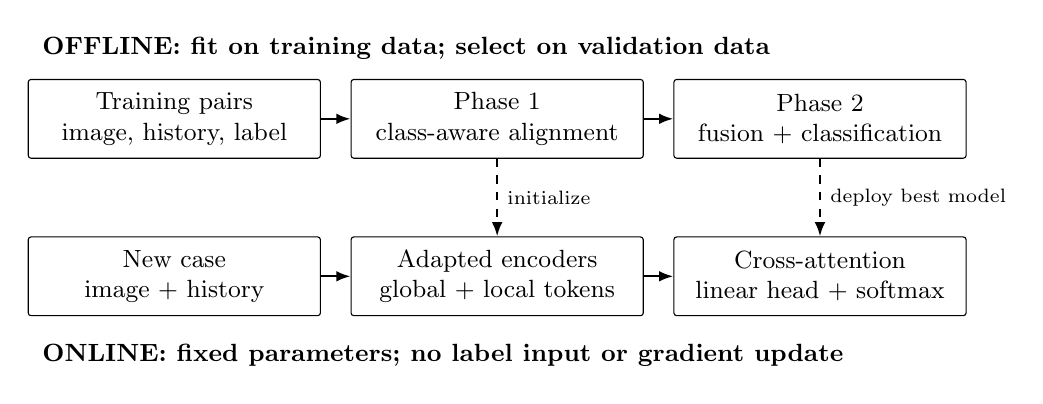
\begin{tikzpicture}[font=\small,
 box/.style={draw,rounded corners=1pt,align=center,minimum height=10mm,text width=35mm,inner sep=3pt},
 arr/.style={-{Latex[length=1.8mm]},thick}]
\node[box] (data) at (0,0) {Training pairs\\image, history, label};
\node[box] (p1) at (4.1,0) {Phase 1\\class-aware alignment};
\node[box] (p2) at (8.2,0) {Phase 2\\fusion + classification};
\draw[arr] (data)--(p1); \draw[arr] (p1)--(p2);
\node[box] (new) at (0,-2.0) {New case\\image + history};
\node[box] (enc) at (4.1,-2.0) {Adapted encoders\\global + local tokens};
\node[box] (pred) at (8.2,-2.0) {Cross-attention\\linear head + softmax};
\draw[arr] (new)--(enc); \draw[arr] (enc)--(pred);
\draw[arr,dashed] (p1)--node[right,font=\scriptsize]{initialize}(enc);
\draw[arr,dashed] (p2)--node[right,font=\scriptsize]{deploy best model}(pred);
\node[font=\small\bfseries,anchor=west] at (-1.8,0.9) {OFFLINE: fit on training data; select on validation data};
\node[font=\small\bfseries,anchor=west] at (-1.8,-3.0) {ONLINE: fixed parameters; no label input or gradient update};
\end{tikzpicture}
}
\caption{Offline learning and online prediction. Phase 1 initializes the encoders used in Phase 2; the final deployment contains their Phase-2-adapted weights together with fusion and classification. Dashed arrows indicate learned-state transfer.}
\label{fig:framework}
\end{figure}

For CTCH, the text includes the reason for admission, disease history, and prior medical history, using their prepared English translations. Imaging findings, the professional diagnosis, and the target label are excluded from the text input. Labels are used only for offline supervision and evaluation. BTXRD has no natural paired history; its text is generated from metadata and is therefore analyzed separately. This distinction is part of the evaluation protocol rather than an assumed equivalence between text sources.

\subsection{Representations and Low-Rank Adaptation}
Each radiograph is passed through the native BiomedCLIP resize, center-crop, and normalization transform to obtain a $224\times224$ RGB image. The visual transformer uses $16\times16$ patches. Its projected output consists of one global token $v_0$ and 196 patch tokens $V_\ell$, each of dimension $d=512$. The PubMedBERT-based text branch uses up to 256 token positions and projects them to the same dimension. In Phase 2, $t_0$ denotes the first projected text token and $T_\ell$ the remaining tokens. Padding positions are masked. The original pooled image and text representations are used for Phase-1 matching; these pooled outputs should not be confused with the token-level fusion inputs.

For a pretrained matrix $W_0\in\mathbb R^{d_o\times d_i}$, LoRA computes
\begin{equation}
Wx=W_0x+\frac{\alpha}{r}BAx,
\quad A\in\mathbb R^{r\times d_i},\ B\in\mathbb R^{d_o\times r}.
\label{eq:lora}
\end{equation}
The base matrix remains fixed. The encoder adapter rank is $r=16$, scaling is $\alpha=32$, and dropout is 0.1. Adapters are inserted into attention projections and feed-forward linear layers of both encoders. For one matrix, the update uses $r(d_i+d_o)$ parameters instead of $d_id_o$. The complete model also trains the fusion and classifier; consequently, the overall trainable ratio must be measured rather than inferred from rank alone.

\subsection{Phase 1: Class-Aware Soft Semantic Matching}
The principle is to reduce conflicting supervision from same-class examples while retaining patient-specific correspondence. For a batch of size $B$, define the unnormalized affinity
\begin{equation}
S_{ij}=\begin{cases}
1,&i=j,\\
\rho,&i\ne j\ \text{and}\ y_i=y_j,\\
0,&\text{otherwise},
\end{cases}\qquad \rho=0.5.
\label{eq:target}
\end{equation}
Normalize each row to obtain $Q^{I\to T}_{ij}=S_{ij}/\sum_kS_{ik}$. The reverse target is the row-normalized transpose of $Q^{I\to T}$. With unit-normalized pooled embeddings $\bar v_i,\bar t_j$, the logits and directional probabilities are
\begin{equation}
C_{ij}=e^s\bar v_i^\top\bar t_j,
\quad P^{I\to T}_{ij}=\frac{e^{C_{ij}}}{\sum_k e^{C_{ik}}},
\quad P^{T\to I}=\operatorname{softmax}_{\rm row}(C^\top),
\label{eq:contrastive}
\end{equation}
where $s$ is the pretrained logit scale, fixed in this LoRA configuration. The symmetric objective is
\begin{equation}
\mathcal L_1=-\frac{1}{2B}\sum_{i,j}\left[
Q^{I\to T}_{ij}\log P^{I\to T}_{ij}+
Q^{T\to I}_{ij}\log P^{T\to I}_{ij}\right].
\label{eq:loss1}
\end{equation}
Class-aware sampling groups at least two examples of a selected class, making off-diagonal positive mass available within a minibatch. If a row has $m$ same-class partners, its true pair receives $1/(1+\rho m)$ and each partner $\rho/(1+\rho m)$. If $m=0$, the target reduces to ordinary one-pair matching. For one directional cross-entropy, the logit derivative is proportional to $P_{ij}-Q_{ij}$; thus, the optimizer no longer unconditionally pushes every unmatched same-class example away. This explains the intended learning behavior without asserting that class equality captures every clinical similarity.

\subsection{Phase 2: Global-to-Local Fusion and Classification}
The principle is conditional evidence selection: the global image queries text tokens, while the global text queries image patches. After separate input layer normalization and linear projection, define a single attention head as
\begin{equation}
\operatorname{Att}(Q,K,V;M)=
\operatorname{softmax}\left(\frac{QW_Q(KW_K)^\top}{\sqrt{d_h}}+M\right)VW_V,
\label{eq:attention}
\end{equation}
where $M$ is zero on valid keys and negative infinity on padding. Eight heads are concatenated and projected to form $\operatorname{MHA}$. The bidirectional residual updates are
\begin{align}
h_I&=\operatorname{LN}\left(v_0+\operatorname{Drop}(\operatorname{MHA}(v_0,T_\ell,T_\ell;M_T))\right),\\
h_T&=\operatorname{LN}\left(t_0+\operatorname{Drop}(\operatorname{MHA}(t_0,V_\ell,V_\ell;0))\right).
\label{eq:bidirectional}
\end{align}
Separate global layer normalizations precede these queries. Concatenation, a $1024\to512\to512$ MLP with GELU and dropout, and output layer normalization produce
\begin{equation}
z=\operatorname{LN}(\operatorname{MLP}([h_I;h_T])),\quad
\ell=W_cz+b_c,\quad p=\operatorname{softmax}(\ell).
\label{eq:classifier}
\end{equation}
The linear head has $K(512+1)$ parameters. Cross-attention is asymmetric in query and key length: each global query selects context from a local sequence. The attention matrix therefore grows linearly with the number of local keys, although encoder self-attention still contributes its usual computational cost. This construction uses patch tokens from one transformed image; it does not process extra high-resolution crops.

To account for the long tail, let $n_c$ be the number of training examples in class $c$. Effective-number weights \cite{Cui2019ClassBalanced} are normalized across present classes and capped:
\begin{equation}
a_c=\frac{1-\beta}{1-\beta^{n_c}},\qquad
w_c=\min\left(\frac{Ka_c}{\sum_j a_j},5\right),\qquad\beta=0.999.
\label{eq:weights}
\end{equation}
With smoothing $\epsilon=0.1$, $u_{ic}=(1-\epsilon)\mathbf1[y_i=c]+\epsilon/K$. The implementation uses weighted, smoothed cross-entropy with mean reduction:
\begin{equation}
\mathcal L_2=-\frac{\sum_{i=1}^{B}\sum_{c=1}^{K}w_cu_{ic}\log p_{ic}}
{\sum_{i=1}^{B}w_{y_i}}.
\label{eq:loss2}
\end{equation}
Adapters remain trainable in Phase 2 together with fusion and the linear head; the pretrained base weights remain frozen. Smoothing places nonzero mass on every class, so the class weights also affect those off-target terms. This specifies the actual objective more precisely than multiplying a smoothed loss by the target-class weight alone.

\subsection{Algorithms and Interpretation}
Algorithm~\ref{alg:training} separates fitting, validation selection, and online use. Classification uses the softmax argmax; no confidence calibration is required for the reported labels.

\begin{table}[t]
\caption{Algorithm 1: Offline fitting and online prediction}
\label{alg:training}
\begin{tabularx}{\textwidth}{@{}rY@{}}
\toprule
1 & \textbf{Input:} fixed training/validation partitions, pretrained encoders, class map, and hyperparameters. \\
2 & Construct permitted history text and native image transforms. Insert LoRA; freeze base encoder weights. \\
3 & \textbf{Phase 1:} sample class-aware batches; compute pooled features, $S$, $Q$, and $\mathcal L_1$; update adapters. Retain the checkpoint with minimum validation loss. \\
4 & \textbf{Phase 2:} initialize from retained adapters; expose image/text tokens; build bidirectional attention and a linear head. Compute training-only $w_c$. \\
5 & For each minibatch, evaluate Eqs.~\eqref{eq:attention}--\eqref{eq:loss2} and update adapters, fusion, and classifier. Retain maximum validation Macro-F1. \\
6 & \textbf{Output:} final weights, class ordering, preprocessing/tokenizer settings, and configuration. \\
\midrule
7 & \textbf{Online input:} a new radiograph $x$ and corresponding history $t$; apply the saved transforms. \\
8 & Extract native tokens; compute $z$, $\ell$, and $p$ using fixed weights. \\
9 & Return $\widehat y=\arg\max_c p_c$ and class scores. No labels, optimization, or test-time fitting are used. \\
\bottomrule
\end{tabularx}
\end{table}

Scientifically, C1 specifies cross-modal conditioning and C2 uses class identity to shape representations. Practically, LoRA reduces optimized weights. The ablations test alignment and fusion, but do not isolate every loss and sampling component.

\section{Experimental Results}
\subsection{Purposes, Datasets, and Protocol}
Table~\ref{tab:questions} maps experiments to contributions. The primary endpoint is Macro-F1; accuracy and balanced accuracy provide complementary views. For class $c$, $\mathrm{F1}_c=2TP_c/(2TP_c+FP_c+FN_c)$, with zero for an undefined value, and Macro-F1 averages it over $K$ classes. Balanced accuracy averages $TP_c/(TP_c+FN_c)$. Neither metric is a substitute for examining rare-class support.

\begin{table}[t]
\caption{Experiment purposes and the contributions they assess}
\label{tab:questions}
\small
\begin{tabularx}{\textwidth}{@{}p{12mm}YY@{}}
\toprule
Link & Purpose and comparison & Evidence and interpretation \\
\midrule
C1, C3 & Compare the complete model with six trained baselines on both datasets & Accuracy, balanced accuracy, Macro-F1; paired CTCH comparisons \\
C1, C2 & Compare the full system with Phase 2 only and concatenation & Component-associated differences; confidence intervals and adjusted tests \\
C1 & Compare multimodal training with the image-only control & Descriptive modality/configuration comparison; not a pure text-removal effect \\
C3 & Compare XBone-Net and fully tuned BiomedCLIP resources & Trainable/total parameters, batch-one compute and timing \\
\bottomrule
\end{tabularx}
\end{table}

CTCH contains 3,249 de-identified radiograph--history pairs from 22 classes at a single orthopedic hospital in Ho Chi Minh City. Its fixed patient-grouped split contains 2,265 training, 315 validation, and 669 test examples. The manifest has no patient key shared across partitions, and the test set contains 669 distinct patients. Normal cases constitute 1,086 examples overall, illustrating the skew toward common classes. The text is restricted to the clinical fields described in Section 3.1. Translation fidelity and undocumented history remain possible sources of error.

BTXRD \cite{Yao2025} contains 3,746 radiographs, represented here as one normal class and nine tumor classes. We use 2,621 training, 375 validation, and 750 test images. The split is at image level because the supplied metadata do not provide stable patient identifiers. The generated text uses metadata, including disease-group-dependent construction rules. It can therefore carry label-correlated information. BTXRD evaluates a synthetic-text setting rather than natural-history generalization, and its results must not be read as a second-center validation of CTCH.

The datasets have independently trained models and different label spaces. Seeds 42, 123, and 456 vary training randomness while retaining each dataset's fixed split. Tables report mean $\pm$ sample standard deviation ($n=3$); the standard deviation is not a confidence interval. Prediction archives are aligned by image identifier, ground-truth agreement is checked, and accuracy, balanced accuracy, and Macro-F1 are recomputed from the saved predictions. Where older metric summaries disagree, the aligned archives are used consistently for descriptive and paired comparisons.

Training uses AdamW, cosine scheduling, physical batches of 16, one accumulation step, and BF16 on an NVIDIA GeForce RTX 5060 Ti. Phase 1 permits 30 epochs at $5\times10^{-5}$ with patience 3; Phase 2 permits 50 at $10^{-4}$ with patience 5. Weight decay is $10^{-4}$. The fully tuned BiomedCLIP baseline uses a learning rate of $2\times10^{-5}$ and a global-concatenation classifier. CNN baselines are image-only; CLIP, MedCLIP, PubMedCLIP, and BiomedCLIP baselines use image--text fusion. Thus, baseline comparisons assess complete adaptation recipes, not only encoder quality.

For CTCH, the stored statistical protocol uses 10,000 paired, class-stratified patient-cluster bootstrap replicates crossed with seed resampling for percentile 95\% intervals. Its two-sided permutation test uses 10,000 draws, patient-level model swaps shared across seeds, and seed resampling. Holm adjustment is applied within each metric: six comparisons in the baseline family and two in the architecture family. These are separate analysis families, not a single adjustment over all endpoints. Our current recomputation verifies the descriptive means entering those stored analyses; it does not rerun the resampling draws.

\subsection{Comparison with Other Methods}
\begin{table}[t]
\caption{Recomputed classification results on fixed test partitions, mean $\pm$ sample SD over three seeds. All entries are local trained baselines, not results copied from their original papers.}
\label{tab:classification}
\centering\small
\begin{tabular}{@{}lccc@{}}
\toprule
Model & Accuracy & Balanced accuracy & Macro-F1 \\
\midrule
\textit{CTCH: $N=669$} & & & \\
ResNet-50 & $0.4983\pm0.0077$ & $0.4180\pm0.0046$ & $0.4154\pm0.0020$\\
DenseNet-121 & $0.4818\pm0.0038$ & $0.4920\pm0.0465$ & $0.4360\pm0.0242$\\
CLIP & $0.5874\pm0.0209$ & $0.6217\pm0.0359$ & $0.5633\pm0.0090$\\
MedCLIP & $0.5600\pm0.0396$ & $0.5723\pm0.0177$ & $0.5161\pm0.0224$\\
PubMedCLIP & $0.5521\pm0.0234$ & $0.5589\pm0.0614$ & $0.5203\pm0.0264$\\
BiomedCLIP & $0.5969\pm0.0253$ & $0.6023\pm0.0234$ & $0.5540\pm0.0080$\\
XBone-Net & $0.6183\pm0.0203$ & $0.5935\pm0.0134$ & $0.5727\pm0.0193$\\
\midrule
\textit{BTXRD: $N=750$} & & & \\
ResNet-50 & $0.6067\pm0.0133$ & $0.3180\pm0.0131$ & $0.3285\pm0.0096$\\
DenseNet-121 & $0.6320\pm0.0013$ & $0.3694\pm0.0150$ & $0.3718\pm0.0173$\\
CLIP & $0.8036\pm0.0273$ & $0.5957\pm0.0160$ & $0.5787\pm0.0252$\\
MedCLIP & $0.8209\pm0.0147$ & $0.6127\pm0.0238$ & $0.6057\pm0.0153$\\
PubMedCLIP & $0.7884\pm0.0285$ & $0.6089\pm0.0342$ & $0.5723\pm0.0577$\\
BiomedCLIP & $0.8311\pm0.0028$ & $0.6062\pm0.0254$ & $0.5994\pm0.0124$\\
XBone-Net & $0.8302\pm0.0098$ & $0.6115\pm0.0140$ & $0.6240\pm0.0118$\\
\bottomrule
\end{tabular}
\end{table}

Table~\ref{tab:classification} shows the highest observed CTCH accuracy and Macro-F1 for XBone-Net, at 0.6183 and 0.5727. CLIP has higher balanced accuracy (0.6217 versus 0.5935), so no model dominates every classification measure. Relative to fully tuned BiomedCLIP, XBone-Net gains 0.0187 Macro-F1 and 0.0214 accuracy but loses 0.0088 balanced accuracy. Table~\ref{tab:paired} shows that its Macro-F1 advantage over BiomedCLIP is not statistically established: the interval crosses zero and adjusted $p=0.7105$.

The larger Macro-F1 differences from the two CNN baselines are supported within the specified comparison family, as are differences from MedCLIP and PubMedCLIP. However, CNN comparisons also change modality availability. Those contrasts cannot attribute the gain to the biomedical initialization, LoRA, or fusion mechanism individually. The comparison with CLIP is particularly informative: its Macro-F1 is close to ours and the paired evidence remains inconclusive, despite a different pretraining domain.

On BTXRD, XBone-Net obtains the highest observed Macro-F1 (0.6240). BiomedCLIP has slightly higher accuracy (0.8311 versus 0.8302), and MedCLIP slightly higher balanced accuracy (0.6127 versus 0.6115). The Macro-F1 gain over BiomedCLIP is 0.0246. The contrast between accuracy near 0.83 and Macro-F1 near 0.62 indicates that the class imbalance remains relevant. Because text is generated from label-correlated metadata, this experiment supports performance in the defined synthetic setting, not a claim that the model recovers equivalent information from real histories.

\begin{table}[t]
\caption{CTCH paired Macro-F1 comparisons. $\Delta=$XBone-Net minus comparator. Intervals are unadjusted paired 95\% bootstrap intervals; $p_H$ is Holm-adjusted within each family.}
\label{tab:paired}
\centering\small
\begin{tabular}{@{}lrrr@{}}
\toprule
Comparator & $\Delta$ & 95\% interval & $p_H$ \\
\midrule
ResNet-50 & .1573 & [.1106, .2068] & .0006 \\
DenseNet-121 & .1367 & [.0835, .1878] & .0006 \\
CLIP & .0094 & [$-$.0340, .0514] & .7105 \\
MedCLIP & .0566 & [.0066, .1107] & .0272 \\
PubMedCLIP & .0524 & [.0089, .0985] & .0423 \\
BiomedCLIP & .0187 & [$-$.0192, .0570] & .7105 \\
\midrule
Phase 2 only & .0230 & [$-$.0196, .0665] & .2918 \\
Concatenation & .0250 & [$-$.0109, .0609] & .2918 \\
\bottomrule
\end{tabular}
\end{table}

\subsection{Comparison with Internal Alternatives}
\begin{table}[t]
\caption{CTCH internal comparisons on the same 669 test cases. Mean $\pm$ sample SD over three seeds. Image only also disables Phase 1 and multimodal fusion.}
\label{tab:ablation}
\centering\small
\begin{tabular}{@{}lccc@{}}
\toprule
Configuration & Accuracy & Balanced accuracy & Macro-F1 \\
\midrule
XBone-Net & $0.6183\pm0.0203$ & $0.5935\pm0.0134$ & $0.5727\pm0.0193$\\
Phase 2 only & $0.6004\pm0.0085$ & $0.5552\pm0.0341$ & $0.5497\pm0.0184$\\
Concatenation & $0.5825\pm0.0038$ & $0.5983\pm0.0268$ & $0.5477\pm0.0162$\\
Image only & $0.4439\pm0.0689$ & $0.4843\pm0.0136$ & $0.3813\pm0.0551$\\
\bottomrule
\end{tabular}
\end{table}

Removing Phase 1 lowers mean Macro-F1 from 0.5727 to 0.5497, while substituting concatenation lowers it to 0.5477 (Table~\ref{tab:ablation}). These observations agree with the motivation for semantic initialization and conditional fusion. They do not prove that both components are required: both Macro-F1 intervals in Table~\ref{tab:paired} include zero. The concatenation comparison also improves balanced accuracy slightly, consistent with a trade-off in the distribution of class-wise errors.

For concatenation, the accuracy difference favors XBone-Net by 0.0359, with a 95\% interval [0.0025, 0.0688]. Nevertheless, the adjusted permutation $p=0.0518$ does not pass the 0.05 threshold. This is not a contradiction: the interval is unadjusted and the test uses a different inferential construction plus multiplicity correction. We therefore avoid interpreting the interval alone as confirmatory evidence for the architecture.

The image-only control obtains Macro-F1 $0.3813\pm0.0551$, 0.1914 below the full system. Clinical information is associated with a substantial benefit in the tested recipes. However, the control removes text, the alignment phase, and the fusion module. It does not isolate text availability under an otherwise unchanged optimization path. A text-only control and controlled history replacement would be needed to distinguish complementary information from reliance on history. We do not import values from older, incompatible runs to fill those missing comparisons.

These experiments assess C1 and selected parts of C2. No dedicated removal of class-aware sampling, same-class target mass, class weights, or smoothing is evaluated here. Consequently, the results do not establish that the proposed recipe solves minority-class imbalance or that any one of those ingredients causes the observed improvement.

\subsection{Parameter and Inference Costs}
\begin{table}[t]
\caption{CTCH resource comparison at seed 42. Parameter counts include the adaptation model. Inference measurements are batch-one averages over repeated forwards; FLOPs use the repository's profiling convention.}
\label{tab:resources}
\centering\small
\begin{tabular}{@{}lrr@{}}
\toprule
Quantity & BiomedCLIP (full tuning) & XBone-Net \\
\midrule
Total parameters & 196,439,831 & 204,348,695 \\
Trainable parameters & 196,439,831 & 8,445,974 \\
Trainable / total & 100.00\% & 4.13\% \\
GFLOPs & 81.032 & 82.318 \\
Throughput (samples/s) & 75.6 & 64.1 \\
Latency (ms) & 13.77 & 16.17 \\
GPU memory (MiB) & 770.7 & 782.5 \\
\bottomrule
\end{tabular}
\end{table}

XBone-Net trains 8.45M of 204.35M parameters on CTCH, approximately 4.13\% (Table~\ref{tab:resources}). Relative to 196.44M trainable parameters in the full-tuning baseline, this is approximately a 95.7\% reduction in optimized weights. The trainable subset consists of 5,013,504 adapter parameters, 3,421,184 fusion parameters, and 11,286 classifier parameters. For BTXRD the smaller head yields 8,439,818 trainable parameters out of 204,342,539.

This supports parameter efficiency, not a smaller total model or faster inference. The seed-42 profile uses BF16 on the RTX 5060 Ti, 20 batch-one inputs, 10 warm-up forwards per input, and 10 timed repeats per input. LoRA is merged for inference. Timings exclude data loading and device transfer; supported-operation FLOPs count a multiply-add as two operations. XBone-Net has lower throughput and higher latency. A smaller trainable state therefore trades off against inference cost.

\section{Limitations and Conclusion}
The strongest evidence is an observed combination of competitive fixed-split classification and a substantially smaller trainable parameter set. The architecture comparisons support plausible mechanisms but leave their incremental Macro-F1 effects statistically unresolved. Three training seeds describe optimization variability on one partition; they do not measure uncertainty across hospitals or alternative data splits. Rare-class performance remains a concern, and there is no fully factorial ablation of the imbalance treatment.

CTCH is a private single-center cohort. Its documentation states that the data were de-identified and used for research under a confidentiality agreement; the source records cannot be publicly released. Institutional approval or exemption details and the authorization for publication must be finalized by the authors before submission. BTXRD is public, but its image-level split and synthetic histories limit patient-level and clinical interpretation. No prospective evaluation, radiologist study, or patient-outcome analysis is included.

XBone-Net reaches Macro-F1 of 0.5727 on CTCH and 0.6240 on BTXRD while updating about 4.13\% of parameters. The resulting adaptation recipe warrants independent validation, history-corruption tests, and targeted loss/sampler ablations before stronger methodological or clinical claims.

\subsubsection{Acknowledgements and AI Assistance.}
OpenAI Codex assisted preparation of the Abstract and Sections 1--5, including prose drafting, source checking, table-generation code, and the schematic. Experimental predictions were taken from existing research artifacts; no training runs were generated for manuscript preparation. Responsibility for the submitted content and final verification rests with the authors.

\subsubsection{Disclosure of Interests.}
Author declarations of financial and non-financial interests are pending confirmation for this draft.

\bibliographystyle{splncs04}
\bibliography{references}
\end{document}
